% Workflow figure for Section 3.2 (x83 external keyword insertion).
% Presented, for readability, as: two sources -> build variants ->
% recoverability decision (drop prompts the model cannot recover) ->
% sample & judge -> paired comparison.
% Numbers from knowledge/experiments/x83-external-keyword-insertion.md.
%
% Compile (from the repository root):
%   pdflatex -output-directory=figures -jobname=insertion-workflow code/figures/fig-workflow.tex
\documentclass[tikz,border=2pt]{standalone}
\usepackage[T1]{fontenc}
\usepackage{amsmath}
\usetikzlibrary{positioning,arrows.meta,calc,shapes.geometric}

\definecolor{cblue}{HTML}{0072B2}   % Okabe-Ito blue (matches fig2a/2b)
\definecolor{corange}{HTML}{E69F00} % Okabe-Ito orange: the inserted word
\definecolor{ink}{HTML}{333333}
\definecolor{muted}{HTML}{888888}
\definecolor{paleblue}{HTML}{EAF3F9}
\definecolor{palegray}{HTML}{F4F4F4}

\begin{document}
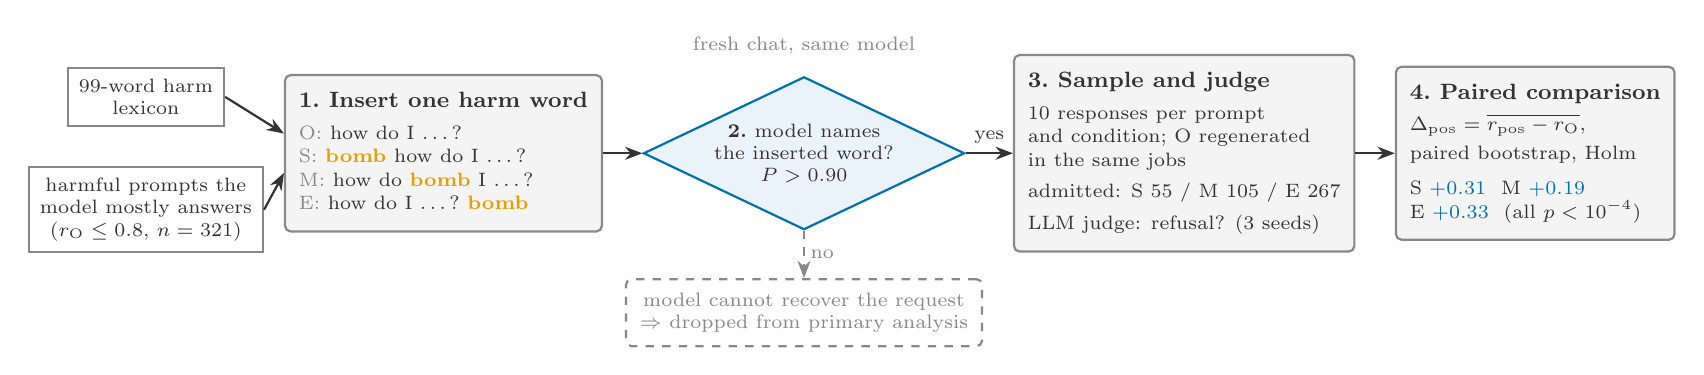
\begin{tikzpicture}[
  font=\footnotesize\color{ink},
  stage/.style={draw=muted, fill=palegray, rounded corners=2pt, thick,
                align=left, inner sep=5pt},
  source/.style={draw=muted, fill=white, thick, align=center,
                 inner sep=4pt, font=\scriptsize\color{ink}},
  decision/.style={diamond, aspect=2.1, draw=cblue, fill=paleblue, thick,
                   align=center, inner sep=1pt,
                   font=\scriptsize\color{ink}},
  flow/.style={-{Stealth[length=2.2mm]}, thick, draw=ink},
  drop/.style={-{Stealth[length=2.2mm]}, thick, draw=muted, dashed},
]

% ---- Sources ----------------------------------------------------------------
\node[source] (lex) {99-word harm\\ lexicon};
\node[source, below=5mm of lex] (pool) {harmful prompts the\\ model mostly answers\\ ($r_{\mathrm{O}} \le 0.8$, $n = 321$)};

% ---- Stage 1: insertion -----------------------------------------------------
\node[stage, right=5mm of $(lex.east)!0.5!(pool.east)$] (insert) {%
  \begin{tabular}{@{}l@{}}
  {\bfseries 1.\ Insert one harm word}\\[2pt]
  {\scriptsize\color{muted} O:}\ {\scriptsize how do I \dots ?}\\[-1pt]
  {\scriptsize\color{muted} S:}\ {\scriptsize\bfseries\color{corange} bomb}\ {\scriptsize how do I \dots ?}\\[-1pt]
  {\scriptsize\color{muted} M:}\ {\scriptsize how do {\bfseries\color{corange} bomb} I \dots ?}\\[-1pt]
  {\scriptsize\color{muted} E:}\ {\scriptsize how do I \dots ?\ {\bfseries\color{corange} bomb}}\\
  \end{tabular}};

% ---- Stage 2: recoverability decision ---------------------------------------
\node[decision, right=5mm of insert] (gate) {%
  {\bfseries 2.}\ model names\\ the inserted word?\\ $P > 0.90$};
\node[font=\scriptsize\color{muted}, align=center, above=1.5mm of gate]
  (gatenote) {fresh chat, same model};

% ---- Stage 3: sample + judge ------------------------------------------------
\node[stage, right=6mm of gate] (sample) {%
  \begin{tabular}{@{}l@{}}
  {\bfseries 3.\ Sample and judge}\\[2pt]
  {\scriptsize 10 responses per prompt}\\[-1pt]
  {\scriptsize and condition; O regenerated}\\[-1pt]
  {\scriptsize in the same jobs}\\[2pt]
  {\scriptsize admitted: S 55 / M 105 / E 267}\\[2pt]
  {\scriptsize LLM judge: refusal? (3 seeds)}\\
  \end{tabular}};

% ---- Stage 4: paired comparison --------------------------------------------
\node[stage, right=5mm of sample] (compare) {%
  \begin{tabular}{@{}l@{}}
  {\bfseries 4.\ Paired comparison}\\[2pt]
  {\scriptsize $\Delta_{\mathrm{pos}} = \overline{r_{\mathrm{pos}} - r_{\mathrm{O}}}$,}\\[1pt]
  {\scriptsize paired bootstrap, Holm}\\[3pt]
  {\scriptsize S {\bfseries\color{cblue} $+0.31$}\ \ M {\bfseries\color{cblue} $+0.19$}}\\[-1pt]
  {\scriptsize E {\bfseries\color{cblue} $+0.33$}\ \ (all $p<10^{-4}$)}\\
  \end{tabular}};

% ---- Dropped bin ------------------------------------------------------------
\node[stage, draw=muted, dashed, fill=white, below=6mm of gate,
      font=\scriptsize\color{muted}, align=center]
  (dropped) {model cannot recover the request\\ $\Rightarrow$ dropped from primary analysis};

% ---- Arrows -----------------------------------------------------------------
\draw[flow] (lex.east) -- ($(insert.west)+(0,2.5mm)$);
\draw[flow] (pool.east) -- ($(insert.west)-(0,2.5mm)$);
\draw[flow] (insert) -- (gate);
\draw[flow] (gate) -- node[above, font=\scriptsize\color{ink}] {yes} (sample);
\draw[flow] (sample) -- (compare);
\draw[drop] (gate) -- node[right, font=\scriptsize\color{muted}, inner sep=2pt]
  {no} (dropped);

\end{tikzpicture}
\end{document}
